%4.1.tex

LLVMにおいて特定のターゲットマシン命令の生成は\ref{chp:3_1}で述べたSelectionDAGISelパスによるSelectフェーズにてLLVM IRの命令からターゲットマシン命令に変換されることによって行われる.
この変換はSelectionDAGのノードに対してパターンマッチングを行い,特定のパターンにターゲット命令を対応させる手法で行われる.

このパターンマッチングに用いるパターンはLLVMの固有ドメイン言語であるTableGenによって行われる.TableGenはターゲットマシンの命令やレジスタ等の情報を記述するために用いられる.TableGenでは命令生成のためにパターンの定義だけでなく,アセンブリコード等の出力のためにニーモニックの定義や命令フォーマットの定義も行っている.

SelectionDAGのパターンマッチングの例を図\ref{fig:SelectionDAG_example}
に示す.
図\ref{fig:SelectionDAG_example}
では加算命令の例を示している.図\ref{fig:SelectionDAG_example}上にパターン定義クラスPatがある.Patクラスの第一引数と変換前のSelectionDAGのノードが一致した場合,Patクラスの第二引数で指定したノードに変換する.

\begin{figure}[bt]
    \centering
    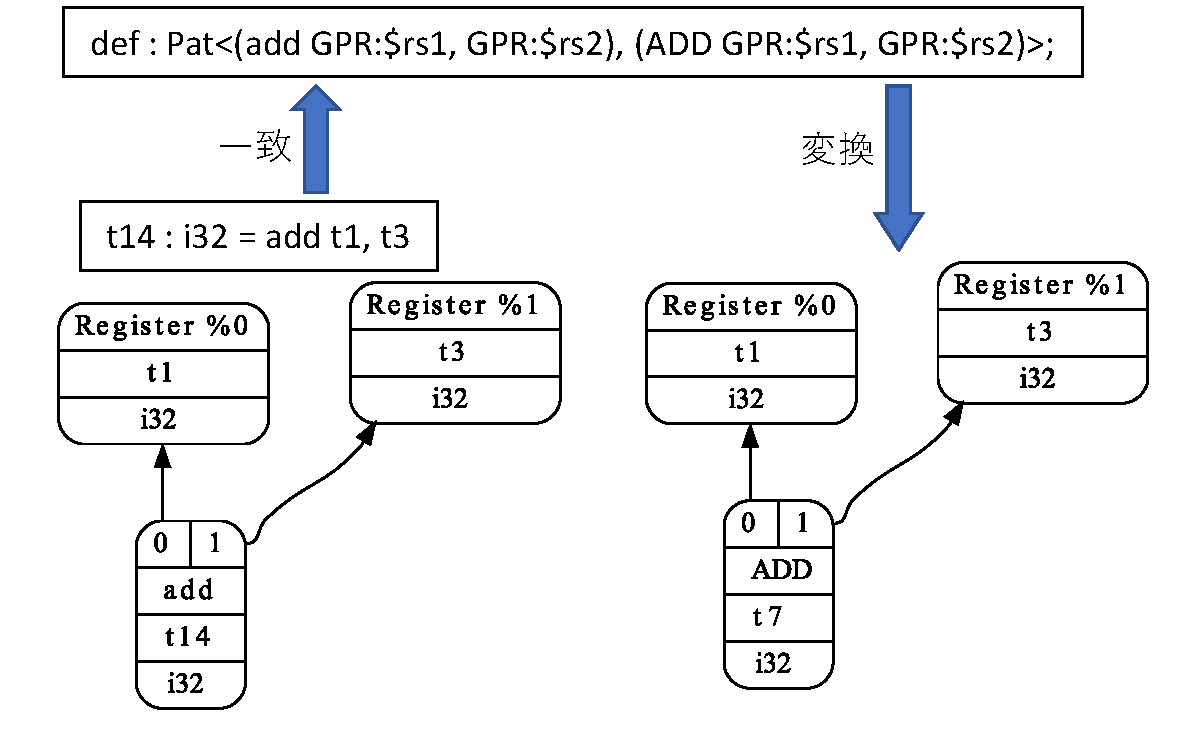
\includegraphics[scale=0.6]{image/SelectionDAG_example.pdf}
    \caption{SelectionDAGの命令変換}
    \label{fig:SelectionDAG_example}
\end{figure}

この様にSelectionDAGのパターンと命令ごとに定義されているパターンが一致したときに対応した命令にノードが変換される.
LLVMではRISC-VのV拡張命令のためのパターン定義が既に実装されており,そのパターンと一致した際に変換する命令を独自のベクトル拡張付きRISC-Vの命令に定義しなおすことによってベクトル拡張付きRISC-V命令の生成を実現する.

LLVMにおける命令の定義は命令フォーマットの定義と命令の定義に分かれる.命令フォーマットはTableGenによって命令の種類ごとにフォーマットのクラスを定義を行う.LLVMにおける命令フォーマットは基本クラスRVInstを継承する形で行われる.RVInstでは32ビットのフィールドInstや命令のニーモニックを格納するAsmStringを定義している.このRVInstを継承して異なるフォーマットを定義していく.

命令の定義は命令フォーマットのクラスをインスタンス化する形で行われるが,そのために命令フォーマットを更に継承したクラスを定義する.このクラスは似たような種類の命令を定義するに当たって同じような定義を何度も繰り返さないように定義する.

命令フォーマット,命令定義のクラスの継承関係を図\ref{fig:InstFromat_class}%図を作り直し、ラップクラスも書く
に示す.基本クラスであるRVInstを継承して基本命令のフォーマットの定義を行っている.クラスALU\_rr,ALU\_riはそれぞれ算術演算命令のためのクラスである.ALU\_rrは汎用レジスタ同士の加算や減算の算術演算の定義に用いられ,ALU\_riは即値を用いた算術演算の命令定義に用いられる.

\begin{figure}[tb]
    \centering
    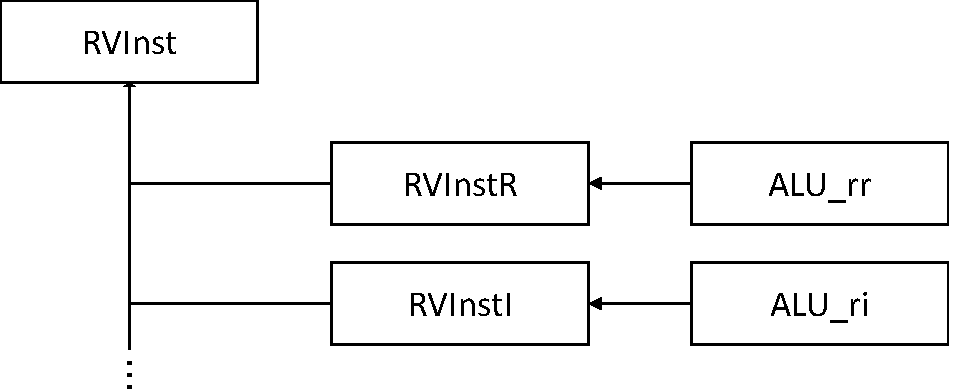
\includegraphics[scale=0.5]{image/InstFormat_class.pdf}
    \caption{基本命令フォーマットクラス継承関係}
    \label{fig:InstFromat_class}
\end{figure}

LLVMでは上記のように命令の定義が行われており,この定義方法に従った形式で我々のベクトル拡張付きRISC-Vのベクトル命令の定義を行う.